\chapter{Background}\label{ch02:litreview}

This chapter provides an overview of time-series forecasting techniques, with a focus on contemporary deep learning approaches, particularly transformer-based models. We also explore the architectures of the state-of-the-art transformer-based time-series forecasting methods which are the subject of comparison, and the recent work on the comparison of transformer-based architectures for time-series forecasting \cite{Wawale2022ANOM, Mendis2024MultivariateTS}.

\section{Deep Learning in Time-Series Forecasting}\label{sec:tsforecasting}

In recent years, deep learning techniques have emerged as powerful alternatives to traditional methods, largely due to their ability to model nonlinear relationships and capture intricate temporal dependencies. Models such as Long Short-Term Memory (LSTM) networks, Gated Recurrent Units (GRUs), and other Recurrent Neural Network (RNN)-based architectures have demonstrated considerable success in various domains, including time-series prediction \cite{Wang2024AdvancementsID, Kumar2024ASO}. These models excel at automatically learning feature representations from raw data, which is particularly beneficial when dealing with high-dimensional and noisy time-series datasets \cite{Abbas2024DeepLT}. 

LSTMs, for example, address the vanishing gradient problem inherent in traditional RNNs by introducing memory cells and gating mechanisms, enabling them to capture long-term dependencies more effectively. Similarly, GRUs simplify the LSTM architecture by combining the forget and input gates into a single update gate, reducing computational complexity while maintaining competitive performance. These advancements have made deep learning a popular choice for time-series forecasting, particularly in applications where traditional methods fall short \cite{Hochreiter1997LongSM}.

\section{Transformers in Deep Learning}\label{sec:transformers}

Transformers were introduced in the seminal work \textit{Attention is All You Need} and have since become the cornerstone of modern deep learning. The key innovation of transformers is the self-attention mechanism, which allows the model to weigh the importance of different parts of the input sequence without relying on recurrence. This mechanism enables transformers to capture long-range dependencies more effectively than traditional RNNs, while also facilitating parallelization during training \cite{Vaswani2017AttentionIA}.

A typical transformer architecture consists of multiple layers of multi-head attention, positional encodings, and feed-forward networks. Multi-head attention allows the model to focus on different parts of the input sequence simultaneously, while positional encodings provide information about the order of elements in the sequence. These components work together to enable transformers to model complex relationships within the data, making them highly versatile and scalable \cite{Vaswani2017AttentionIA}.

\subsection{Transformers in Time-Series Forecasting}

Adapting transformer architectures for time-series forecasting presents unique challenges. Unlike natural language, time-series data often exhibits irregular intervals, varying temporal dynamics, and domain-specific patterns. To address these challenges, researchers have proposed various modifications to standard transformer architectures. For instance, specialized positional encodings have been developed to better capture the temporal structure of time-series data, while tailored attention mechanisms have been introduced to model irregular intervals and long-term dependencies more effectively \cite{kim2024continuoustimelinearpositionalembedding, aguileramartos2024localattentionmechanismboosting}.

Additionally, hybrid architectures that combine transformers with other deep learning components, such as temporal convolutional layers or recurrent networks, have been explored. These hybrid models aim to leverage the strengths of both approaches, enhancing the model's ability to capture complex temporal patterns while maintaining computational efficiency. Despite these advancements, challenges remain, particularly in balancing model complexity with performance and achieving robust results across different forecasting horizons and data modalities \cite{Liu2024EnhancedTS}.

\section{Specific Transformer-Based Models}\label{sec:specificmodels}

In this section, we provide a detailed overview of the four transformer-based models examined in this paper: SAMFormer, TimesFM, TimeGPT and Time-MoE. Each model represents a unique approach to time-series forecasting,since they each leverage different architectural innovations and pre-training strategies.

\subsection{SAMFormer}

SAMFormer is a lightweight transformer architecture specifically designed for long-term multivariate time-series forecasting. The model employs a shallow transformer encoder, which reduces computational complexity while maintaining competitive performance. A key feature of SAMFormer is its use of channel-wise attention, which captures inter-feature correlations in multivariate data. This is particularly important in scenarios where multiple time-series variables influence each other, such as in financial or energy forecasting \cite{ilbert2024samformerunlockingpotentialtransformers}.

\begin{figure}[ht]
    \centering
    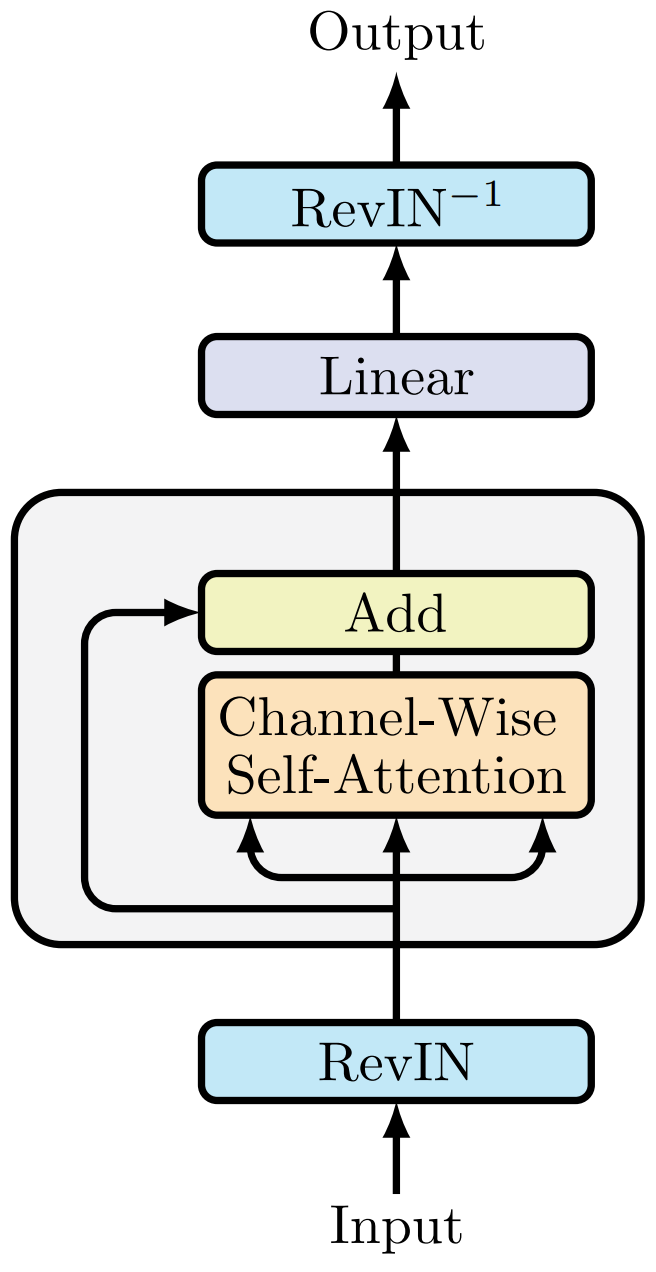
\includegraphics[width=3cm, height=6cm]{figures/samformer.PNG}
    \caption{SAMFormer Architecture \cite{ilbert2024samformerunlockingpotentialtransformers}}
    \label{fig:samformer}
\end{figure}

Another distinctive aspect of SAMFormer is its integration of Reversible Instance Normalization (RevIN), a technique that mitigates the distribution shift between training and testing phases. By normalizing the input data in a reversible manner, RevIN ensures that the model generalizes well to unseen data. Additionally, SAMFormer incorporates Sharpness-Aware Minimization (SAM), an optimization technique that drives the model toward flatter minima in the loss landscape. This enhances the model's generalization performance, making it particularly effective for long-term forecasting tasks \cite{Kim2022ReversibleIN}.

\subsection{TimesFM}

TimesFM is a decoder-only foundation model developed for univariate time-series forecasting. The model processes time-series data in patches, typically consisting of 32 time points, and is pre-trained on a mixture of synthetic and real-world datasets. The synthetic data is generated from simulations or statistical models, while the real-world data includes large-scale datasets such as Google Trends and Wikipedia Pageviews. This extensive pre-training enables TimesFM to perform zero-shot forecasting, allowing it to generalize to new datasets without additional task-specific training \cite{das2024decoderonlyfoundationmodeltimeseries}.

\begin{figure}[ht]
    \centering
    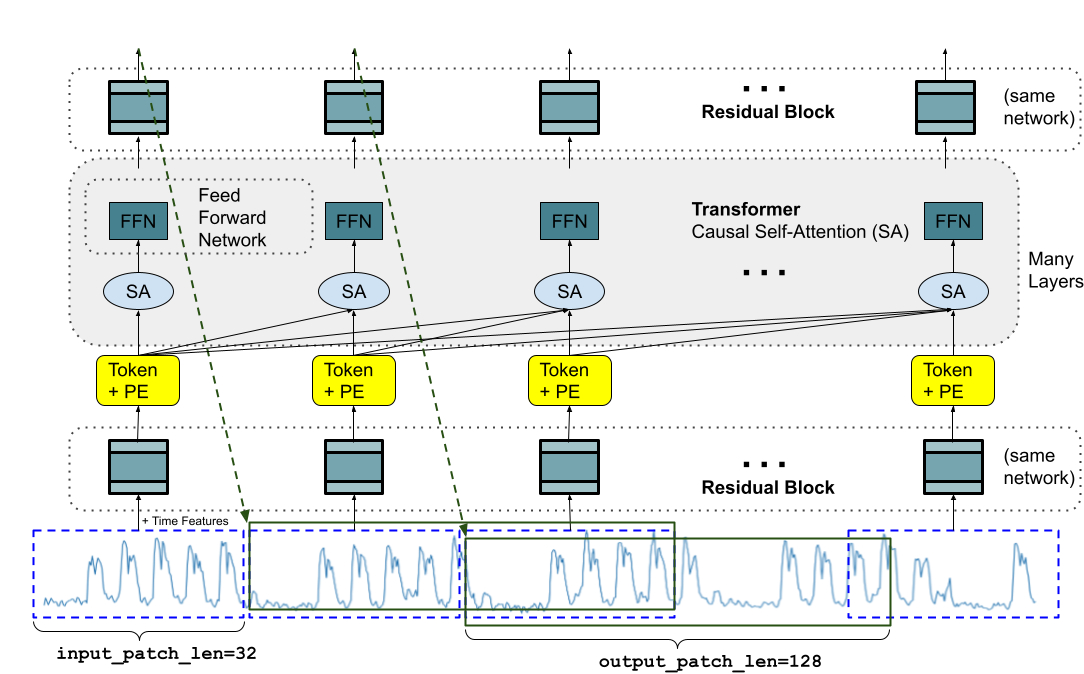
\includegraphics[width=11cm, height=7cm]{figures/timesfm.jpg}
    \caption{TimesFM Architecture \cite{das2024decoderonlyfoundationmodeltimeseries}}
    \label{fig:timesfm}
\end{figure}

TimesFM's decoder-only architecture contributes to its computational efficiency and flexibility. The model can be fine-tuned on specific datasets to further enhance its performance, making it a versatile choice for a wide range of forecasting applications. Its ability to achieve competitive performance in zero-shot settings is particularly noteworthy, as it reduces the need for large amounts of labeled data, which is often a bottleneck in time-series forecasting \cite{das2024decoderonlyfoundationmodeltimeseries}.

\subsection{Time-MoE}

Time-MoE is a family of decoder-only time-series foundation models that leverage a mixture-of-experts (MoE) architecture to achieve scalable forecasting performance. The model scales up to 2.4 billion parameters and is trained on a massive dataset comprising over 300 billion time points across nine different domains. This extensive pre-training allows Time-MoE to handle arbitrary context and prediction lengths, making it highly adaptable to diverse forecasting scenarios \cite{Shi2025TimeMoE}.

The mixture-of-experts framework in Time-MoE dynamically allocates computational resources across different subsets of the input, enhancing the model's ability to capture intricate temporal patterns \cite{Shi2025TimeMoE}. This is particularly beneficial in applications that require high scalability and adaptability, such as financial market forecasting or energy demand prediction \cite{Wang2023VE}. Time-MoE's ability to model complex temporal dynamics across multiple domains makes it a powerful tool for real-world forecasting tasks \cite{Shi2025TimeMoE}.

\subsection{TimeGPT}

TimeGPT utilizes a transformer-based architecture with self-attention mechanisms, structured in an encoder-decoder format comprising multiple layers enhanced by residual connections and layer normalization. This design enables the model to effectively process historical data and generate accurate forecasts. A linear layer maps the decoder's output to the forecasting window's dimensions, facilitating precise predictions. TimeGPT is capable of handling various input sizes and forecasting horizons, adapting to different time-series characteristics \cite{Garza2023TimeGPT}.

Trained on the largest collection of publicly available time-series datasets at the time of training, encompassing over 100 billion data points from domains such as finance, healthcare, and IoT sensor data, TimeGPT captures a wide array of temporal patterns. In empirical evaluations, TimeGPT's zero-shot inference demonstrated superior performance, efficiency, and simplicity compared to established statistical, machine learning, and deep learning methods \cite{Garza2023TimeGPT}. These results underscore its robustness and versatility in time-series forecasting applications.


\section{Broader Evaluations and Surveys}

Beyond individual model introductions, recent works have evaluated Transformer forecasters more generally. Below, an overview of research papers comparing transformer-based architectures for time-series forecasting is provided.

Meyer et al. (2024) benchmarked foundation models (Chronos, TimesFM, LagLlama) against task-specific Transformer models for short-term electricity load forecasting~\cite{meyer2024benchmarking}. They found that large pre-trained models perform comparably to specialized Transformers, and in fact, TimesFM outperforms all trained-from-scratch models when provided a sufficiently long input window~\cite{meyer2024benchmarking}. Crucially, the foundation models achieved this with zero-shot inference (no retraining), highlighting the practical advantages of minimal tuning effort~\cite{meyer2024benchmarking}.

Kim et al. (2024) provide a comprehensive survey of modern time-series forecasting, noting the rise of Transformers and foundation models in the field~\cite{kim2024survey}. They discuss how earlier simple models sometimes rivaled Transformers, but the newest innovations—including hybrid architectures and large pre-trained models—are driving a “renaissance” in forecasting research~\cite{kim2024survey}. This aligns with the emergence of SAMformer, TimeGPT, TimesFM, and Time-MoE, which collectively represent the latest trends: improving core Transformer training and scaling models via massive data pre-training.

These studies illustrate both the potential and limitations of transformer-based architectures in time-series forecasting. While foundation models demonstrate competitive performance and practical advantages like zero-shot inference, their improvements over specialized models are often marginal and highly dependent on dataset characteristics. The reliance on large-scale pre-training raises questions about efficiency and accessibility, particularly for domains with limited data. In the following methodology section, we outline the experimental setup, evaluation criteria, and datasets used to systematically compare these models.